%! TeX program = lualatex
%tags! mapas de karnaugh mapas
\documentclass[letterpaper]{article}
\usepackage[margin=1in]{geometry}
\usepackage{amsmath}
\usepackage{amssymb}
\usepackage{circuitikz}
\usepackage[no-math]{fontspec}
\usepackage[fg,bg]{gruvboxpalette}
\usepackage{hyperref}
\usepackage{newtxsf}
\usepackage[explicit]{titlesec}
\usepackage{tikz}
\usetikzlibrary{calc}
\usetikzlibrary{positioning}
\usetikzlibrary{arrows.meta}
\usepackage[most]{tcolorbox}
\usepackage{tabularray}
\DefTblrTemplate{firsthead, middlehead,lasthead}{default}{}
\DefTblrTemplate{capcont}{default}{}
\DefTblrTemplate{contfoot-text}{normal}{} \SetTblrTemplate{contfoot-text}{normal} \DefTblrTemplate{conthead-text}{normal}{} \SetTblrTemplate{conthead-text}{normal}
\UseTblrLibrary{counter}
\hypersetup{
  colorlinks  = true,
  urlcolor    = Blue,
  linkcolor   = Blue,
  citecolor   = Blue
}
\usepackage[most]{tcolorbox}

\setmainfont{NotoSans-Regular}[
Path           = /home/snouflake/.fonts/ ,
Extension      = .ttf ,
BoldFont       = NotoSans-Bold ,
ItalicFont     = NotoSans-Italic ,
BoldItalicFont = NotoSans-BoldItalic,
] 

\newtcolorbox{defbox}[3][]{%
  colback=blue!30!background,
  coltitle=blue!15!black,
  coltext=font,
  title filled=false,
	enhanced,
  detach title,
  tile,
  before upper={\tcbtitle\medskip\\},
  borderline west={2mm}{0pt}{blue},
  % attach boxed title to top center={yshift=-2mm},
  leftrule=2mm,
  toprule=0mm,
  bottomrule=0mm,
  rightrule=0mm,
  arc=0mm,
	title={Definición:~#2},
	#1
}

\setlength\parindent{0pt}

\usepackage[italic]{mathastext}

\def \T{Sistemas Digitales}
\def \S{Mapas de Karnaugh}

\begin{document}
\begin{tikzpicture}[inner sep=0pt,color=font]
  \node[anchor=west,align=left,line width=0pt] 
    (title) at (0,0) {\huge\bfseries\noindent\T\\\Large\bfseries\S}
    ;
\end{tikzpicture}


\begin{longtblr}{
    colspec={@{}Q[3cm,cmd=\textbf,h] >{\begin{minipage}{\linewidth}}X<{\end{minipage}}@{}},
    rowsep={7pt}
  }
  Dos variables
  &
  Para una función $f(A,B)$, su mapa de Karnaugh es
  \medskip

  \begin{center}
    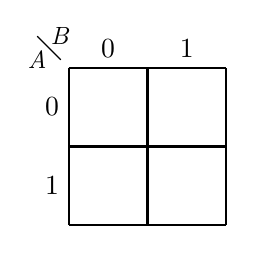
\begin{tikzpicture}
      % \node[anchor=south east] at (0,0) {$A \textbackslash B$};
      \draw (-0.1,0.1) -- (-0.4,0.4);
      \node[inner sep=0pt,anchor=center] at (-0.4,0.1) {\small{$A$}};
      \node[inner sep=0pt,anchor=center] at (-0.1,0.4) {\small{$B$}};
      \draw[step=1cm,thick] (0,0) grid (2,-2);
      \node[anchor=south] at (0.5,0) {$0$};
      \node[anchor=south] at (1.5,0) {$1$};
      \node[anchor=east] at (0,-0.5) {$0$};
      \node[anchor=east] at (0,-1.5) {$1$};
    \end{tikzpicture}
  \end{center}
  
  donde cada espacio tiene un 1 si $f$ se evalúa a 1 con los valores de $A$ y $B$ que representa.
  \\
  &
  Sea $y = \bar{B}A + BA$.

  \begin{center}
    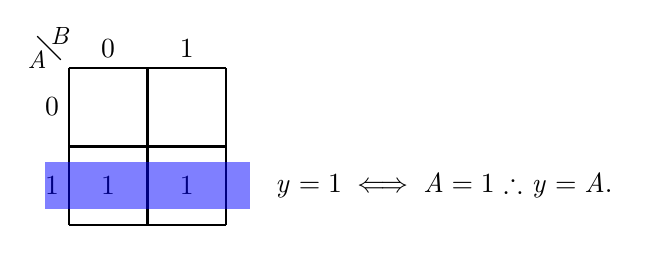
\begin{tikzpicture}
      % \node[anchor=south east] at (0,0) {$A \textbackslash B$};
      \draw (-0.1,0.1) -- (-0.4,0.4);
      \node[inner sep=0pt,anchor=center] at (-0.4,0.1) {\small{$A$}};
      \node[inner sep=0pt,anchor=center] at (-0.1,0.4) {\small{$B$}};
      \draw[step=1cm,thick] (0,0) grid (2,-2);
      \node[anchor=south] at (0.5,0) {$0$};
      \node[anchor=south] at (1.5,0) {$1$};
      \node[anchor=east] at (0,-0.5) {$0$};
      \node[anchor=east] at (0,-1.5) {$1$};

      \node at (0.5,-0.5) {};
      \node at (1.5,-0.5) {};
      \node at (0.5,-1.5) {1};
      \node at (1.5,-1.5) {1};

      \fill[blue,opacity=0.5] (-0.3,-1.2) rectangle (2.3,-1.8);

      \node[anchor=west] at (2.5,-1.5) {$y = 1 \iff A = 1$ $\therefore$ $y = A$.};
    \end{tikzpicture}
  \end{center}
  \\
  &
  Sea $y = \bar{B}\bar{A} + B\bar{A} + BA$.

  \begin{center}
    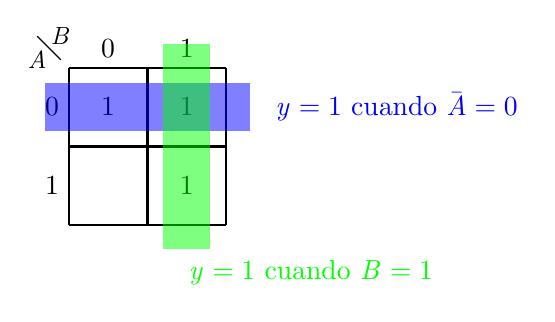
\begin{tikzpicture}
      \draw (-0.1,0.1) -- (-0.4,0.4);
      \node[inner sep=0pt,anchor=center] at (-0.4,0.1) {\small{$A$}};
      \node[inner sep=0pt,anchor=center] at (-0.1,0.4) {\small{$B$}};
      \draw[step=1cm,thick] (0,0) grid (2,-2);
      \node[anchor=south] at (0.5,0) {$0$};
      \node[anchor=south] at (1.5,0) {$1$};
      \node[anchor=east] at (0,-0.5) {$0$};
      \node[anchor=east] at (0,-1.5) {$1$};

      \node at (0.5,-0.5) {1};
      \node at (1.5,-0.5) {1};
      \node at (0.5,-1.5) {};
      \node at (1.5,-1.5) {1};

      \fill[blue,opacity=0.5] (-0.3,-0.2) rectangle (2.3,-0.8);
      \fill[green,opacity=0.5] (1.2,0.3) rectangle (1.8,-2.3);

      \node[anchor=west] at (2.5,-0.5) {\color{blue}{$y = 1$ cuando $\bar{A} = 0$}};
      \node[anchor=west] at (1.4,-2.6) {\color{green}{$y = 1$ cuando $B = 1$}};
    \end{tikzpicture}
    \vspace{-15pt}

    $$\therefore y = \textcolor{blue}{\bar{A}} + \textcolor{green}{B}$$
  \end{center}
  \\
  Tres variables
  &
  Es importante tomar en cuenta que el mapa de tres variables se comporta como un anillo; las columnas en ambos extremos horizontales se pueden asociar, en este caso como $\bar{b}$.
  \begin{center}
    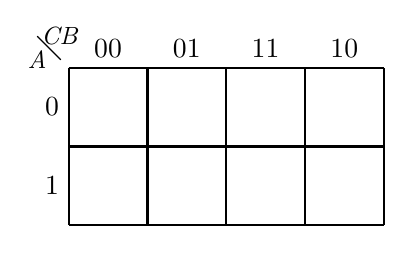
\begin{tikzpicture}
      \draw (-0.1,0.1) -- (-0.4,0.4);
      \node[inner sep=0pt,anchor=center] at (-0.4,0.1) {\small{$A$}};
      \node[inner sep=0pt,anchor=center] at (-0.1,0.4) {\small{$CB$}};
      \draw[step=1cm,thick] (0,0) grid (4,-2);
      \node[anchor=south] at (0.5,0) {$00$};
      \node[anchor=south] at (1.5,0) {$01$};
      \node[anchor=south] at (2.5,0) {$11$};
      \node[anchor=south] at (3.5,0) {$10$};
      \node[anchor=east] at (0,-0.5) {$0$};
      \node[anchor=east] at (0,-1.5) {$1$};

      \node at (0.5,-0.5) { };
      \node at (1.5,-0.5) { };
      \node at (2.5,-0.5) { };
      \node at (3.5,-0.5) { };
      \node at (0.5,-1.5) { };
      \node at (1.5,-1.5) { };

      % \fill[blue,opacity=0.5] (-0.3,-0.2) rectangle (2.3,-0.8);
      % \fill[green,opacity=0.5] (1.2,0.3) rectangle (1.8,-2.3);
      %
      % \node[anchor=west] at (2.5,-0.5) {\color{blue}{$y = 1$ cuando $\bar{A} = 0$}};
      % \node[anchor=west] at (1.4,-2.6) {\color{green}{$y = 1$ cuando $B = 1$}};
    \end{tikzpicture}
    \vspace{-15pt}

    % $$\therefore y = \textcolor{blue}{\bar{A}} + \textcolor{green}{B}$$
  \end{center}
  \\
  &
  Sea $f(C,B,A) = \bar{C} \bar{B} \bar{A} + \bar{C} B \bar{A} + \bar{C} B A + C \bar{B} \bar{A} + C \bar{B} A + C B A$.
  \begin{center}
    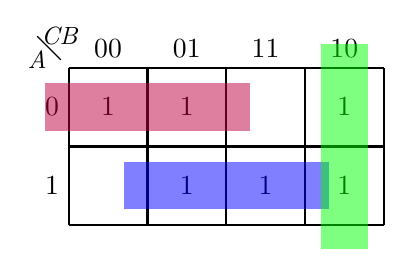
\begin{tikzpicture}
      \draw (-0.1,0.1) -- (-0.4,0.4);
      \node[inner sep=0pt,anchor=center] at (-0.4,0.1) {\small{$A$}};
      \node[inner sep=0pt,anchor=center] at (-0.1,0.4) {\small{$CB$}};
      \draw[step=1cm,thick] (0,0) grid (4,-2);
      \node[anchor=south] at (0.5,0) {$00$};
      \node[anchor=south] at (1.5,0) {$01$};
      \node[anchor=south] at (2.5,0) {$11$};
      \node[anchor=south] at (3.5,0) {$10$};
      \node[anchor=east] at (0,-0.5) {$0$};
      \node[anchor=east] at (0,-1.5) {$1$};

      \node at (0.5,-0.5) {1};
      \node at (1.5,-0.5) {1};
      \node at (2.5,-0.5) { };
      \node at (3.5,-0.5) {1};
      \node at (0.5,-1.5) { };
      \node at (1.5,-1.5) {1};
      \node at (2.5,-1.5) {1};
      \node at (3.5,-1.5) {1};

      \fill[purple,opacity=0.5] (-0.3,-0.2) rectangle (2.3,-0.8);
      \fill[blue,opacity=0.5] (0.7,-1.2) rectangle (3.3,-1.8);
      \fill[green,opacity=0.5] (3.2,0.3) rectangle (3.8,-2.3);
    \end{tikzpicture}
    \vspace{-15pt}

    $$
    \therefore y = 
    \textcolor{purple}{\bar{C}\bar{A}} +
    \textcolor{blue}{BA} + 
    \textcolor{green}{C \bar{B}}
    $$
  \end{center}

\end{longtblr}

\section*{Multiplexers}

\begin{longtblr}{
    colspec={@{}Q[3cm,cmd=\textbf,h] >{\begin{minipage}{\linewidth}}X<{\end{minipage}}@{}},
    rowsep={7pt}
  }
  2 x 1 
  &
  \begin{circuitikz}[american,thick]
    \draw
    (1,-2) node[not port, rotate=-90, scale=0.5, anchor=out] (snot) {}
    (0,0) node[above] (S) {S} to[short,-*] ++(0,-3) coordinate (sw) to ++(0,-2)
    (0,0) to (1,0) to (snot.in)
    (snot.out) to (1,-5)

    (2,0) node[above] (A) {A} to[short,-*] ++(0,-1) coordinate (aw) to ++(0,-4)
    (3,0) node[above] (B) {B} to[short,-*] ++(0,-4) coordinate (bw) to ++(0,-1)

    (4,-1.5) node[and port, anchor=west] (and1) {}
    (4,-3.5) node[and port, anchor=west] (and2) {}

    (aw) -| (and1.in 1)
    (snot.out) -| (and1.in 2)

    (sw) -| (and2.in 1)
    (bw) -| (and2.in 2)

    (6,-2.5) node[or port, anchor=west] (or1) {}
    (or1.out) node[right] {X}

    (and1.out) -| (or1.in 1)
    (and2.out) -| (or1.in 2)

    (9,-2.5) node[dipchip, hide numbers, num pins=4, anchor=west] (dc) {}
    (dc.bpin 1) node[right, font=\small] {A}
    (dc.bpin 2) node[right, font=\small] {B}
    (dc.bpin 3) node[left, font=\small] {S}
    (dc.bpin 4) node[left, font=\small] {X}
    ;
  \end{circuitikz}
  \\
  8 x 1
  &
  \begin{circuitikz}[american, thick]
    \draw
    (0,0) node[dipchip, hide numbers, num pins=16, draw only pins={1-12}] (dc) {}
    (dc.bpin 1) node[right] { 7 }
    (dc.bpin 2) node[right] { 6 }
    (dc.bpin 3) node[right] { 5 }
    (dc.bpin 4) node[right] { 4 }
    (dc.bpin 5) node[right] { 3 }
    (dc.bpin 6) node[right] { 2 }
    (dc.bpin 7) node[right] { 1 }
    (dc.bpin 8) node[right] { 0 }

    (dc.bpin 9) node[left] { X }

    (dc.bpin 10) node[left] { $S_{1}$ }
    (dc.bpin 11) node[left] { $S_{2}$ }
    (dc.bpin 12) node[left] { $S_{3}$ }
    ;
  \end{circuitikz}
  \\
  Mapa $\to$ multiplexer
  &
  
  \begin{circuitikz}[american, thick]
    \node[anchor=north east] at (-1,0) {
      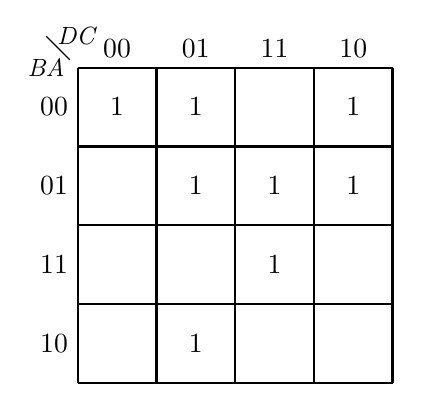
\begin{tikzpicture}
        \draw (-0.1,0.1) -- (-0.4,0.4);
        \node[inner sep=0pt,anchor=center] at (-0.4,0.0) {\small{$BA$}};
        \node[inner sep=0pt,anchor=center] at (-0.0,0.4) {\small{$DC$}};
        \draw[step=1cm,thick] (0,0) grid (4,-4);
        \node[anchor=south] at (0.5,0) {$00$};
        \node[anchor=south] at (1.5,0) {$01$};
        \node[anchor=south] at (2.5,0) {$11$};
        \node[anchor=south] at (3.5,0) {$10$};

        \node[anchor=east] at (0,-0.5) {$00$};
        \node[anchor=east] at (0,-1.5) {$01$};
        \node[anchor=east] at (0,-2.5) {$11$};
        \node[anchor=east] at (0,-3.5) {$10$};

        \node at (0.5,-0.5) {1};
        \node at (1.5,-0.5) {1};
        \node at (2.5,-0.5) { };
        \node at (3.5,-0.5) {1};
        \node at (0.5,-1.5) { };
        \node at (1.5,-1.5) {1};
        \node at (2.5,-1.5) {1};
        \node at (3.5,-1.5) {1};
        \node at (1.5,-3.5) {1};
        \node at (2.5,-2.5) {1};
      \end{tikzpicture}
    }
    ;

    \node[dipchip, hide numbers, num pins=32, draw only pins={1-21}, anchor=west] (dc) at (2,-4.5) {}
    ;
    \draw[thick]
    (dc.bpin 1) node[right]  { 15 }
    (dc.bpin 2) node[right]  { 14 }
    (dc.bpin 3) node[right]  { 13 }
    (dc.bpin 4) node[right]  { 12 }
    (dc.bpin 5) node[right]  { 11 }
    (dc.bpin 6) node[right]  { 10 }
    (dc.bpin 7) node[right]  { 9 }
    (dc.bpin 8) node[right]  { 8 }
    (dc.bpin 9) node[right]  { 7 }
    (dc.bpin 10) node[right] { 6 }
    (dc.bpin 11) node[right] { 5 }
    (dc.bpin 12) node[right] { 4 }
    (dc.bpin 13) node[right] { 3 }
    (dc.bpin 14) node[right] { 2 }
    (dc.bpin 15) node[right] { 1 }
    (dc.bpin 16) node[right] { 0 }

    (dc.bpin 17) node[left] { X }

    (dc.bpin 18) node[left] { $S_{1}$ }
    (dc.bpin 19) node[left] { $S_{2}$ }
    (dc.bpin 20) node[left] { $S_{3}$ }
    (dc.bpin 21) node[left] { $S_{4}$ }
    (dc.pin 18) node[right] { D }
    (dc.pin 19) node[right] { C }
    (dc.pin 20) node[right] { B }
    (dc.pin 21) node[right] { A }
    ;
    \draw[red,thick]
    (0,0) node[above] {+}
    (0,0) to ++(0,-9)

    (0,0 |- dc.pin 1)  to[short,*-] (dc.pin 1)
    % (0,0 |- dc.pin 2)  to[short,*-] (dc.pin 2)
    (0,0 |- dc.pin 3)  to[short,*-] (dc.pin 3)
    (0,0 |- dc.pin 4)  to[short,*-] (dc.pin 4)
    (0,0 |- dc.pin 5)  to[short,*-] (dc.pin 5)
    % (0,0 |- dc.pin 6)  to[short,*-] (dc.pin 6)
    (0,0 |- dc.pin 7)  to[short,*-] (dc.pin 7)
    (0,0 |- dc.pin 8)  to[short,*-] (dc.pin 8)
    % (0,0 |- dc.pin 9)  to[short,*-] (dc.pin 9)
    % (0,0 |- dc.pin 10) to[short,*-] (dc.pin 10)
    % (0,0 |- dc.pin 11) to[short,*-] (dc.pin 11)
    (0,0 |- dc.pin 12) to[short,*-] (dc.pin 12)
    % (0,0 |- dc.pin 13) to[short,*-] (dc.pin 13)
    % (0,0 |- dc.pin 14) to[short,*-] (dc.pin 14)
    % (0,0 |- dc.pin 15) to[short,*-] (dc.pin 15)
    (0,0 |- dc.pin 16) to[short,*-] (dc.pin 16)
    ;
    \draw[blue,thick]
    (1,0) to ++(0,-9) node[ground] {}

    (1,0 |- dc.pin 2)  to[short,*-] (dc.pin 2)
    (1,0 |- dc.pin 6)  to[short,*-] (dc.pin 6)
    (1,0 |- dc.pin 9)  to[short,*-] (dc.pin 9)
    (1,0 |- dc.pin 10) to[short,*-] (dc.pin 10)
    (1,0 |- dc.pin 11) to[short,*-] (dc.pin 11)
    (1,0 |- dc.pin 13) to[short,*-] (dc.pin 13)
    (1,0 |- dc.pin 14) to[short,*-] (dc.pin 14)
    (1,0 |- dc.pin 15) to[short,*-] (dc.pin 15)
    ;
  \end{circuitikz}
  \\
  Mapeo de variables
  &
  \begin{circuitikz}[american, thick]
    \node[anchor=east] at (-1,0) {$f(D,C,B,A) \to f(~ D(C,B,A)~, C, B, A)$};
    \draw (-0.1,0.1) -- (-0.4,0.4);
    \node[inner sep=0pt,anchor=center] at (-0.4,0.0) {\small{$C$}};
    \node[inner sep=0pt,anchor=center] at (-0.0,0.4) {\small{$BA$}};
    \draw[step=1cm,thick] (0,0) grid (4,-2);
    \node[anchor=south] at (0.5,0) {$00$};
    \node[anchor=south] at (1.5,0) {$01$};
    \node[anchor=south] at (2.5,0) {$11$};
    \node[anchor=south] at (3.5,0) {$10$};

    \node[anchor=east] at (0,-0.5) {$0$};
    \node[anchor=east] at (0,-1.5) {$1$};

    \node at (0.5,-0.5) {$D$};
    \node at (1.5,-0.5) {$D$};
    \node at (2.5,-0.5) {$D$};
    \node at (3.5,-0.5) {$D$};
    \node at (0.5,-1.5) {$D$};
    \node at (1.5,-1.5) {$D$};
    \node at (2.5,-1.5) {$D$};
    \node at (3.5,-1.5) {$\bar{D}$};


    \draw
      (-1,-3) node {wait what was this for}
      (-2,-3) coordinate(D) node[above] {D}
      (-1,-4) node[not port, rotate=-90, scale=0.5, anchor=out] (Dnot) {}
      (D) to[short] ++(0,-7) coordinate (Dend)
      (D) to[short] ++(1,0) to[short] (Dnot.in)
      (Dnot.out) to[short] (Dend -| Dnot)

      (0,-5) node[dipchip, hide numbers, num pins=16, draw only pins={1-12}, anchor=north west] (dc) {}
      (dc.bpin 1) node[right] { 7 }
      (dc.bpin 2) node[right] { 6 }
      (dc.bpin 3) node[right] { 5 }
      (dc.bpin 4) node[right] { 4 }
      (dc.bpin 5) node[right] { 3 }
      (dc.bpin 6) node[right] { 2 }
      (dc.bpin 7) node[right] { 1 }
      (dc.bpin 8) node[right] { 0 }

      (dc.bpin 9) node[left] { X }

      (dc.bpin 10) node[left] { $S_{1}$ }
      (dc.bpin 11) node[left] { $S_{2}$ }
      (dc.bpin 12) node[left] { $S_{3}$ }
      (dc.pin 10) node[right] { C }
      (dc.pin 11) node[right] { B }
      (dc.pin 12) node[right] { A }

      (Dnot |- dc.pin 1) to[short,*-] (dc.pin 1)
      (D |- dc.pin 2) to[short,*-] (dc.pin 2)
      (D |- dc.pin 3) to[short,*-] (dc.pin 3)
      (D |- dc.pin 4) to[short,*-] (dc.pin 4)
      (D |- dc.pin 5) to[short,*-] (dc.pin 5)
      (D |- dc.pin 6) to[short,*-] (dc.pin 6)
      (D |- dc.pin 7) to[short,*-] (dc.pin 7)
      (D |- dc.pin 8) to[short,*-] (dc.pin 8)
      ;
  \end{circuitikz}

\end{longtblr}



\end{document}


